%
% File acl2010.tex
%
% Contact  jshin@csie.ncnu.edu.tw or pkoehn@inf.ed.ac.uk
%%
%% Based on the style files for ACL-IJCNLP-2009, which were, in turn,
%% based on the style files for EACL-2009 and IJCNLP-2008...

%% Based on the style files for EACL 2006 by
%%e.agirre@ehu.es or Sergi.Balari@uab.es
%% and that of ACL 08 by Joakim Nivre and Noah Smith

\documentclass[12pt]{article}
\usepackage{cse595}
\usepackage{url}
\usepackage{latexsym}
\usepackage{graphicx}
\usepackage{float}

%\setlength\titlebox{6.5cm}    % You can expand the title box if you
% really have to

\title{TagPandr: Tag expansion for flickr images}

\author{Naresh Pratap Singh\\
  {\tt mail2naresh@gmail.com}  \And
  Rohith Menon\\
  {\tt rohithmenon@gmail.com} \And
  Sandesh Singh\\
  {\tt sandesh247@gmail.com}
  }

\date{}

\begin{document}
\maketitle
\begin{abstract}
We present an automatic method to suggest tags based on the existing tags provided by
users. We use co occurrence statistics and wordnet to suggest tags in addition
to the existing tags, and use visual features to maintain the relevance of
the suggested tags to the image under consideration. We learn the visual features
for tags from Flickr image corpus. Experimental results show that better tags
  are suggested especially when the quality of original tags are low.
\end{abstract}

\section{Introduction}

A large number of photos are now available online, especially with photo sharing sites like
Flickr and Picassa. Annotation of images with relevant tags is a very useful feature especially
for image search, categorization and organization. While there has been advances in content
based analysis of images, scaling image data to web scale is a challenge.

In Flickr, tags are assigned by people who upload the photos. Tags irrelevant to the tasks of
image search and categorization happen to exist in the image tags. For eg: 2011 (the year) is generally
a tag associated with a photo taken on the new year of 2011. Similarly, model of camera is yet
another tag which is very specific to an image and not relevant to the content of it. Apart from
this, bulk upload of photo brings along with it the problem of bulk tagging. Especially for such
uploads, we find that a group of photos are tagged with the same set of tags. Such tagging, although
makes sense for the photo group as a whole, turns out to be irrelevant for many images in the group.
Poorly tagged images and under tagged images are other issues with community tagging.

In this work, we present a method to automatically expand the given tags using text features and
rank the expanded tags with the visual features to highly score those tags which are relevant to
the given image. We present multiple statistics about the suggested tags and also perform human
evaluation to compute the human perceived goodness of the suggested tags.

\section{Related Work}
Tag suggestion as a problem for text has been studied well and is also present
in leading bookmarking sites such as del.icio.us and in certain blogging sites
such as blogger. Techniques for generating personalized tag recommendations for
users of social book-marking sites such as del.icio.us are formulated by
\newcite{jaeschke2008tag} and works of \newcite{Byde2007}. Tag suggestion is
an easier problem for text compared to tag suggestion for images. Tag expansion
and ranking has also been a popular research topic in last few years. With the
explosion of images online on Flickr, Picasa, and Google Images etc., it
became necessary to devise means to
organize and manage images more effectively. Research in contextual analysis of
images \newcite{Carneiro2005}, \newcite{LavrenkoNIPS03} has served as a
motivation to apply those techniques in conjunction with textual analysis of
existing tags to suggest high quality relevant tags.
The combined intelligence of visual notion of an image is expressed in the form
of tags that are associated with images on such photo sharing. Such tags tend to represent contextual information about the image.
For instance, a cat in an image would be tagged by the name of the cat and also the tag \emph{cat}.

Our work is similar to the work of \newcite{Liu:2009:TR:1526709.1526757} who have introduced an approach to rank tags using initial relevance
scores based on probability density estimation. They tune these score based on a random walk model
which models transition probabilities. This approach requires large training set to compute the
probability density function and the random walk model. \newcite{Sevil:2010:ATE:1825050.1825058} also have
proposed a methodology for tag expansion which requires user to assign initial tags. Initial tags
are used to target images using similarity of tags. A list of tags is constructed based on the similar images
which are weighted according to the similarity with the target image. The highest rank tags are used to
expand the tags of target image. This approach uses both visual and textual similarities for expansion of tags.
Their approach assign tags when the photo is uploaded. This method relies heavily on the visual similarity
of images and thus, would mainly work for very similar images.

Our method aims to expand and rank tags simultaneously
using tag co-occurrence and visual features. In contrast to \newcite{Sevil:2010:ATE:1825050.1825058} approach,
our method uses co-occurrence to find similar tags. We believe, tag co-occurence will help us to tag images with
such related tags and thus, improve image search results. This approach is more robust than using visual cues to
get similar images. In addition, the similarity of visual features can be used to find more related tags.

\section{Implementation}
We used James Hays' matlab code to query and download the meta-data for images
in eight categories. We used this meta-data to extract the URLs, and the actual
image download was done on a hadoop cluster to reduce the amount of time
required to download all the images.

The tags we found at flickr are not of very high quality. Consequently, even
searches on flickr for any particular category were not of very relevant either.
To provide our implementation with a good training set, we decided to use an
independent source of images for the chosen categories.
For each category, we performed a Google search to get canonical images for
those categories. We found that for any given keyword, the results returned
by Google were consistently more representative of that category. We used the
most similar Flickr images (based on Euclidean distance of the gist vectors)
for training. This helped us filter flickr images to hopefully more relevant
set of images.

%% THIS IS HERE FOR LAYOUR PURPOSES oNLY

\begin{figure}[h]
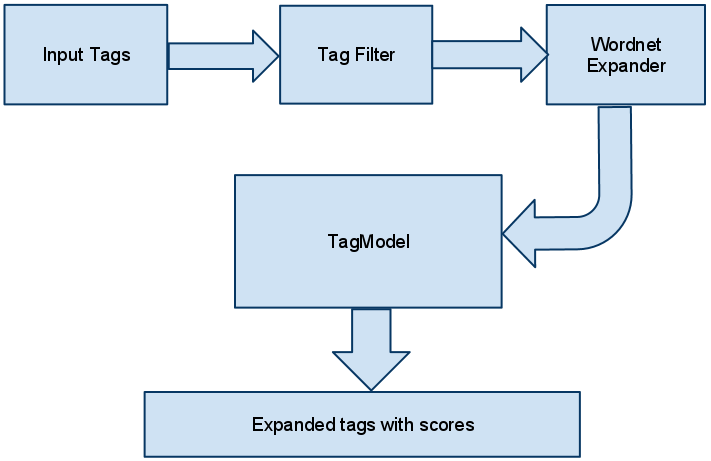
\includegraphics[width=0.5\textwidth]{tagExpansion.png}
\end{figure}

\begin{figure}[h]
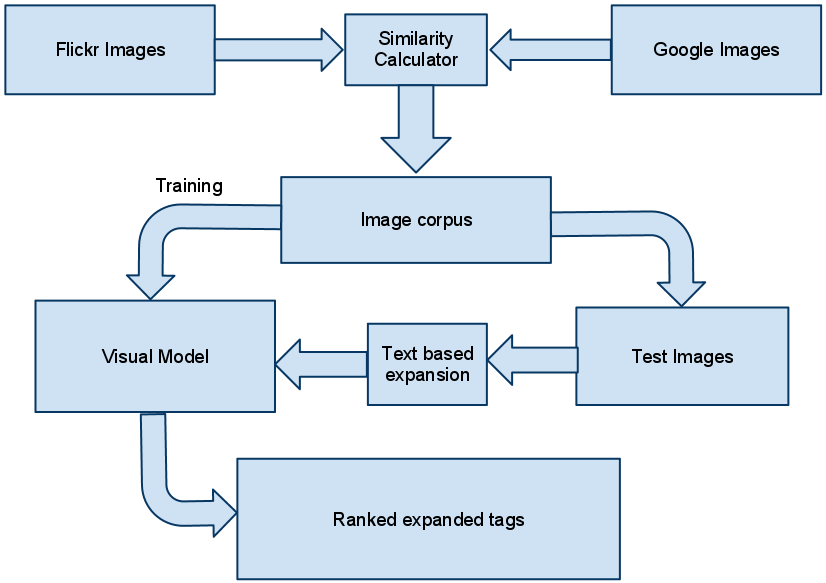
\includegraphics[width=0.5\textwidth]{model.png}
\end{figure}

We trained two models, a tag model and a visual model trained on the visual
features of the images. We filtered the tags such that any word containing
numbers was not considered for training the data. We calculated tag
cooccurence for every pair of tags in the training set, assuming independence
between the pairs. The probability of a given tag  a tag `tag2' depends
on the number of times they co occur with the prior tags. We build a Bayes
model to calculate the probability of seeing a tag given a set of prior tags.
We also extend the list of tags using wordnet \newcite{wordnet}, where we
choose synonyms to augment the original set. Since the text expansion was based
entirely on the prior co-occurrence and wordnet synonyms, we expect this
to give us a very high number of mostly relevant tags. However, some of the words
might be redundant, or even irrelevant -- the visual features are expected
to constrain this set to certain degree of relevance.

We used two visual features, gist vectors and spatial pyramid based on
\newcite{conf/cvpr/LazebnikSP06} method. Gist was expected to help with global features such as
color and environment. The method of spatial pyramid works by partitioning the
image into increasingly fine sub-regions and computing histograms of
local features found inside each sub-region. The resulting ``spatial pyramid''
is a simple and computationally efficient extension of an orderless
bag-of-features image representation, and it
shows significantly improved performance on challenging scene categorization
tasks. We trained multiple classifiers on the visual features by using Weka's
\newcite{hall09} implementation of structure learning of Bayesian networks using
various hill climbing (K2, B, etc) and general purpose (simulated annealing, tabu search)
algorithms.

In spite of the fact that we had a lot of data, unfortunately the machine learning
algorithms themselves were quite slow. Memory and time constraints prevented us from
training using all the data we had, and thus we performed our evaluation on a much
smaller set.


\section{Experimental Evaluation}
We performed experiments on flickr data set. Tags and images were separately downloaded using
flickr apis. We downloaded about 500,000 images from flickr belonging to categories: cat,
dog, train, aircraft, car, bus, places, crocodile, harley etc. We obtained 311,000 unique tags
corresponding to these images. Like mentioned before we filtered tags which contained numbers
and special characters. We found that such tags were not of much relevance to the images.

Evaluation of the tags would require some quantitative way of analyzing quality. We evaluate
the tag quality automatically by two methods. Apart from these automatic methods, we also
perform human evaluation to score the tag quality.

\subsection{Original tag recall in top 5 suggested tags}
In this evaluation, we compute the number of tags in the original image tags that we suggest
in the top five tags automatically suggested by our method. The intuition behind this evaluation
is to make sure that the best tags we suggest have a good coverage of the original tags. Although
this method seems like a good measure of quality, the poor tags present in the original image
will cause this measure to degrade. Our method will fail to suggest original tags if there is
very less relevance with the given image. We calculate this measure of quality for tags generated
with text only features, visual only features and visual + text features. Table \ref{tab:topk} tabulates the
experimental results.


\begin{table*}
  \label{tab:topk}
  \caption{Number of tags in the top 5 predicted tags, present in
  the original}
  \begin{center}
    \begin{tabular}{|l l l l l|}
\hline
Category & Text & Visual & Text + Visual & Total \\
\hline
aircraft & 83 & 41 & 55 & 90 \\
bus & 40 & 13 & 15 & 55 \\
car & 205 & 124 & 111 & 480 \\
cat & 198 & 59 & 64 & 280 \\
crocodile & 89 & 51 & 38 & 100 \\
dog & 110 & 31 & 43 & 145 \\
\hline
\end{tabular}
\end{center}
\end{table*}

From the table its clear that text features alone have better overlap with the given tags.
This is because, the original tags will also be suggested as part of the text co-occurrence
model. We see a decline in the scores with visual only attributes and text+visual attributes.
We attribute this to the fact that for visual features, the ranking of tags comes purely from
the gist or spatial pyramid features and hence the overlap with the original tags will be lesser.
For text+visual features, the ranking of tags push better tags to the top, which has lower overlap
with the original tags compared to text only features.

\subsection{Prediction of original tags removed from test images}
For this evaluation, we randomly remove 30 percent of the original tags from the test images. We
then pass these images through our pipeline and compute the number of tags suggested from the
removed original tags in the top 20 of our suggested tags. The intuition behind this measure of
quality is to understand how well our models are able to simulate the quality of tags possessed
by original tags. This measure also has problems like mentioned before, but is a better measure
of quality because we look for the existence of the removed original tags in the suggested tag
set as a whole. We calculate this measure of quality for tags generated with text only features,
visual only features and visual + text only features. Table \ref{tab:frac} tabulates the experimental results.

\begin{table*}
  \label{tab:frac}
   \caption{Fraction of excluded tags successfully predicted}
\begin{center}
    \begin{tabular}{|l l l l|}
\hline
Category & Text & Visual & Text + Visual \\
\hline
aircraft & 0.87 & 1 & 0.70 \\
bus  & 0.33 & 0.67 & 0.29 \\
car &  0.34 & 0.87 & 0.27 \\
cat &  0.32 & 0.95 & 0.27 \\
crocodile &  0.36 & 1 & 0.34 \\
dog  & 0.29 & 0.89 & 0.22 \\
\hline
\end{tabular}
\end{center}
\end{table*}

% HUMAN EVALUATION
\begin{table*}
  \label{tab:human}
  \caption{Human evaluation}
\begin{center}
    \begin{tabular}{|l l l l l|}
\hline
Category & Text & Visual & Text + Visual & Total \\
\hline
aircraft & 2.05 & 2.07 & 1.95 & 2.13 \\
bus & 2.52 & 2.47 & 2.65 & 2.39 \\
car & 2.26 & 1.80 & 2.41 & 2.43 \\
dogs & 2.64 & 2.13 & 2.57 & 2.53 \\
cats & 3.09 & 2.49 & 3.14 & 2.57 \\
crocodile & 2.79 & 2.08 & 2.36 & 2.59 \\
\hline
\end{tabular}
\end{center}
\end{table*}

\subsection{Evaluation of classifier One Vs Rest}
For this experimental setup, we trained a classifier one for each unique tag appearing at least
10 times in a particular category. We experimented the one vs rest classifier with support vector
machines to learn the visual features for individual tags. It turns out that the performance of
this classifier is worse when compared with a single classifier with multi-class prediction.

\subsection{Human Evaluation}
The above mentioned statistics would provide a notion of quality of the tags suggested. But
we cannot compare it with the quality of the original tags. For this reason, we perform human
evaluation of the input tags for the given image. Human evaluation is performed for each of the
output tag and the original tags. A score from 1 to 4 is assigned to each of the tag, 1 being
lowest on relevance scale and 4 being highest on relevance scale. During evaluation, tags which
were about places and not obvious in the image as part of content were scored as 1. For meta images,
(ie) images which are photos of the writings, visual features will be of very little use. But
text features would prove to be good. Human evaluation was performed for tags expanded with
text only features, visual only features and text+visual features. We also performed human
evaluation of the original tags so that we could compare the scores of the original tags with
the suggested tags. Table \ref{tab:human} tabulates the results of the human evaluation.

\begin{figure*}[t]
\label{fig:graph}
\caption{Human evaluation scores}
\begin{center}
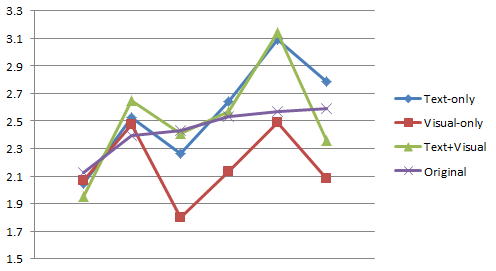
\includegraphics[width=0.8\textwidth]{humanEvalGraph.png}
\end{center}
\end{figure*}


We also found that when the number of tags in the image were less and those ones were very relevant,
the quality of tags expanded tended to be lesser. On the other hand when the original tags were bad,
we were able to suggest better quality tags. We studied the score pattern of original tags with respect
to the suggested tag. Figure \ref{fig:graph} shows scores from text-only, visual-only and text+visual features in
comparison to increasing original tag scores. The graph shows that text+visual and text-only have
higher quality than original tags. Visual-only features, by themselves, although produce lower quality
tags than the original ones, we find that using them in conjunction with text features gives us better
quality than original tags. We can find that text+visual features perform only marginally better than
text only features. We attribute this to the fact that visual model has to learn many classes (tags).
Though the class probabilities from visual classifier are weak representations, it helps in ranking
the text based expanded tags.

\section{Conclusion}
We see that text-based expansion of tags gives us a lot of additional and relevant tags. Our visual classifiers
do not perform as well as we expected them to.

\section*{Acknowledgments}
We thank Professor Tamara Berg for providing us with the insight and support to successfully complete the project.

% you bib file should really go here

\bibliography{bib}
\bibliographystyle{cse595}


\newpage
\section{Examples of generated tags}
\begin{figure}[H]
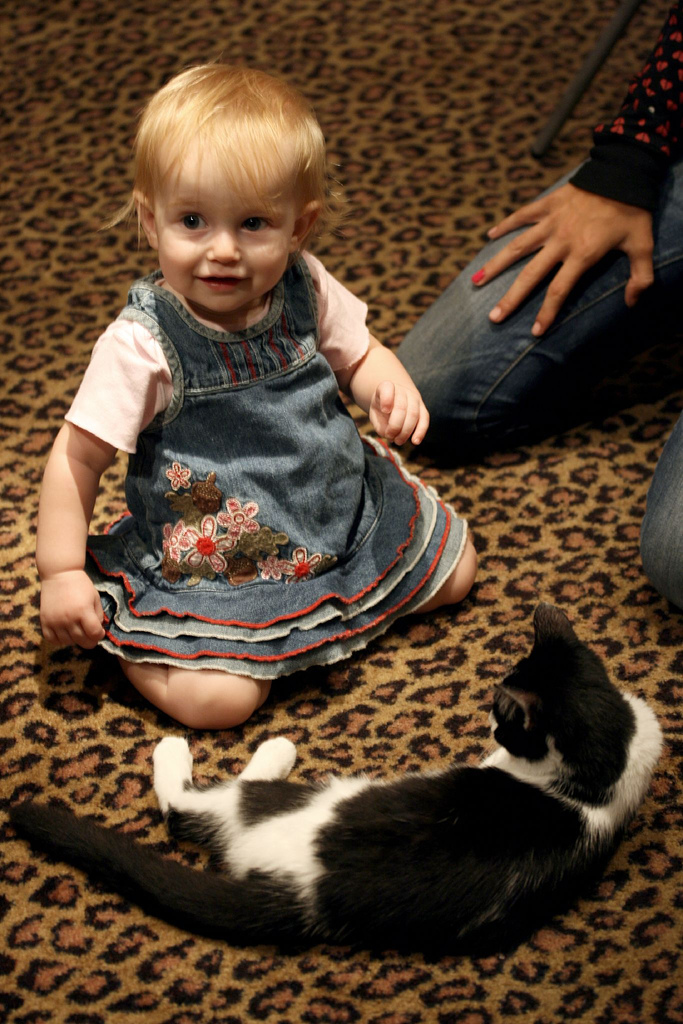
\includegraphics[width=0.5\textwidth]{examples/cat1.jpg}
\end{figure}

\emph{\textbf{Original} cats, baby, cat, person, toddler, sitting, meetup, candid, next, hershey, bpal, willcall, ecwc, nailpolishetc\\
\textbf{Text-only} cats, cat, meetup, hershey, bpal, ecwc, nailpolishetc, willcall, candid, dog, baby, kitty, black, blackness, inkiness, pet, sitting, kitten, cute, pool\\
\textbf{Visual-only} cat, cats, pet, cute, kitten, kitty, animal, pets, home, garden, animals, nature, canon, flowers, family, green, city, dog, flower, car\\
\textbf{Text+Visual} fauna, felid, dogs, girl, baby, black, white, people, street,
house, feline, dog, animals, kitty, animal, kitten, cute, pet, cats, cat}

\begin{figure}[H]
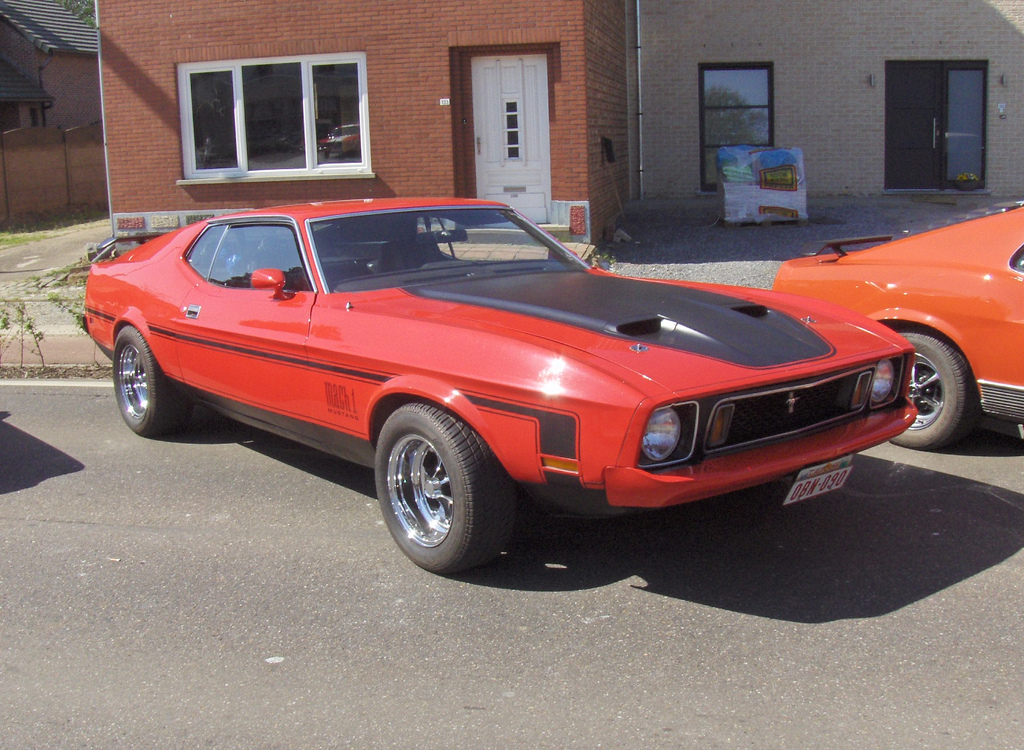
\includegraphics[width=0.5\textwidth]{examples/car2.jpg}
\end{figure}

\emph{\textbf{Original} ford, car, muscle, pony, american, mustang, fever, mustangpassion\\
\textbf{Text-only} car, auto, automobile, machine, motorcar, ford, mustang, muscle, american, pony, mustangpassion, fever, cars, classic, america, us, usa, musculus, carshow, show\\
\textbf{Visual-only} car, show, cars, carshow, auto, truck, club, ford, mustang, race, road, custom, cobra, classic, acctc, alabama, alabamacustomcarandtruckclub, street, chicago, museum\\
\textbf{Text+Visual} muscle, red, american, vintage, blue, racing, automobile, california, usa, street, classic, mustang, race, ford, auto, truck, carshow, cars, show, car
}


\begin{figure}[H]
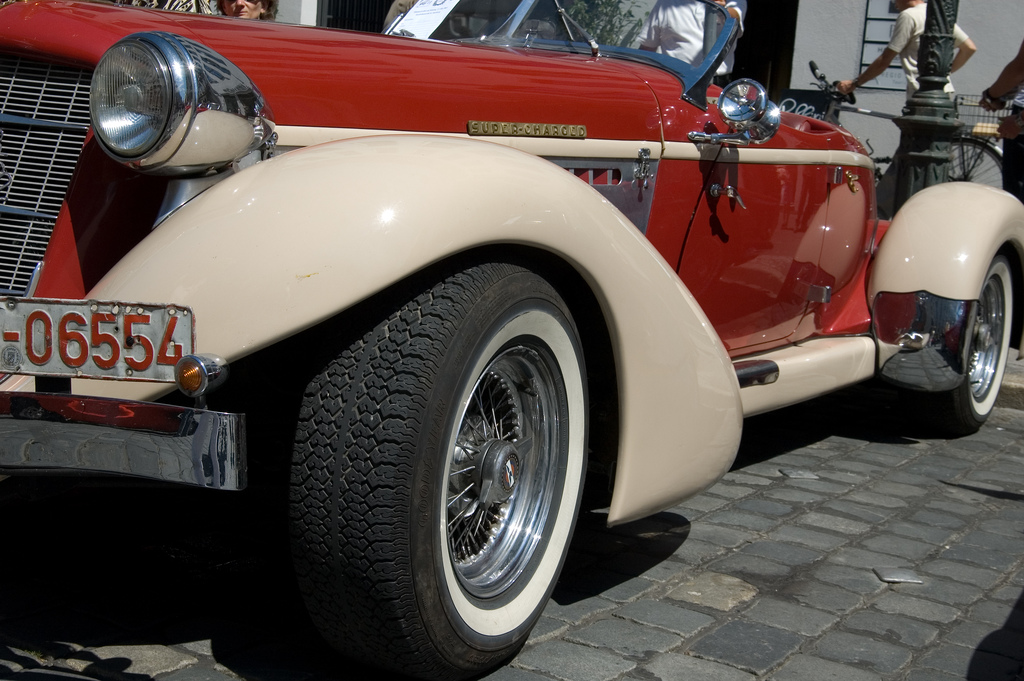
\includegraphics[width=0.5\textwidth]{examples/car1.jpg}
\end{figure}

\emph{\textbf{Original} auto, cars, car, raw, nef, oldtimer, oldcars, augsburg, oldtimershow, muttertag, motherday, maximilianstrasse, moritzplatz, augschburger, borisott, adobelightroom, alteautos, autoschau \\
\textbf{Text-only} cars, oldtimer, car, auto, automobile, machine, motorcar, veteran, stager, warhorse, raw, augsburg, augschburger, borisott, maximilianstrasse, moritzplatz, motherday, muttertag, nef, oldcars \\
\textbf{Visual-only} car, show, cars, carshow, auto, truck, club, ford, mustang, race, road, custom, cobra, classic, acctc, alabama, alabamacustomcarandtruckclub, street, chicago, museum\\
\textbf{Text+Visual} volkswagen, autos, vw, oldtimer, oldcars, red, vintage, antique, mercedes, automobile, street, classic, ford, auto, carshow, cars, car}
\end{document}
